%\documentclass{article}
%\usepackage{graphicx,subfigure}
%\begin{document}

\begin{figure}[!h]
  \centering
   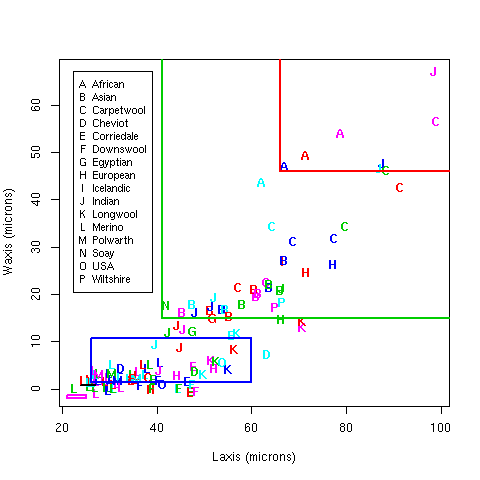
\includegraphics[width=1.0\textwidth]{LWalltypea.png}
  \caption{Plot of breed means of secondary fibre diameter (Ds) and primary fibre diameter (Dp) for 126 flocks sampled by Carter(1968)~\cite{cart:68}. The axes have been rotated 45 degrees so that L-axis represents projections onto the line $D_{p}/D_{s} = 1$, and W-axis represents projections onto a line at right angles to the L-axis. The W-axis is interpreted as two-coatedness, and the L-axis is interpreted as large fibres. The breeds have been grouped into a {\em breed type} which in some cases is an individual breed and in other cases is a country of origin. The coloured rectangles represent  the approximate ranges of L-axis and W-axis values for sheep representing Ryder\'s 4 stages of Merino evolution, plus the modern SRS Fine Merino. Red rectangle is Wild stage, green is Hairy Medium Wool, blue is Generalised Medium Wool, black is Finewool Merino, and magenta is SRS Fine Merino.}
  \label{fig:LWalltypea}
\end{figure}

%\end{document}

